\begin{frame}
\frametitle{WP Apprentissage} 
\begin{minipage}{6cm}
L'objectif de ce groupe de travail est à partir de nombreux exercices, de créer des tactiques spécifiques à ce type d'exercice.
\end{minipage}
\begin{minipage}{4cm}
\includegraphics[scale=0.2]{../images/apprentissage/organisation_apprentissage.pdf}
\end{minipage}

\end{frame}
\begin{frame}


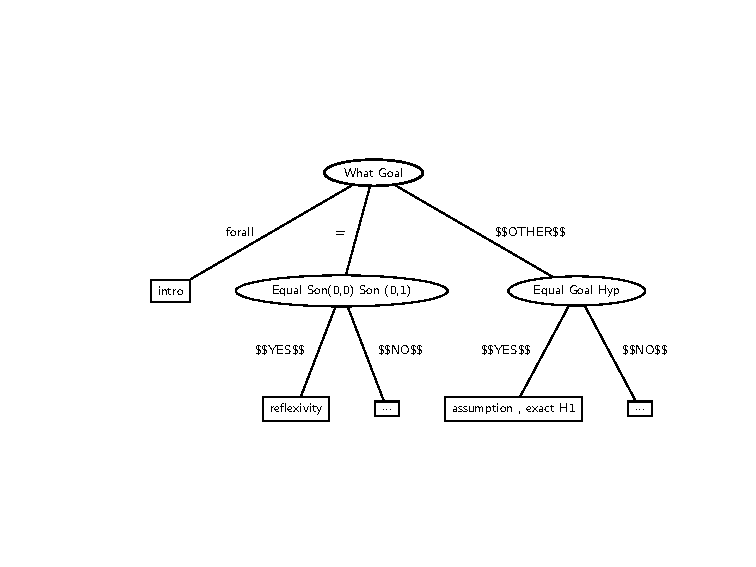
\includegraphics{../images/apprentissage/decision_tree.jpg}

\end{frame}

\begin{frame}

Les questions sont:
\begin{itemize}
    \item Quel est le token à la racine de l'arbre x?
    \item Est-ce que les arbres x et y ont le même token en racine?
\end{itemize}


Pour choisir la question à poser, 
on calcule la question qui nous donne le meilleur rapport "information apportée selon la définition de von Newmann" sur "nombre de réponses". 
On cherche donc à minimiser la taille de l'arbre (et non sa profondeur),
car c'est d'elle que dépend le temps d'exécution et l'occupation de la mémoire.
\end{frame}
\begin{frame}

Résultats
\begin{itemize}
    \item Le parcours d'arbres et le raffinement des données sont utilisables.
    \item L'algorithme d'apprentissage a été réalisé.
\end{itemize}




\end{frame}
